\chapter{Evaluation and Discussion}
\label{chapter:Evaluation}

We first evaluate our approach regarding the obtained results and its performance. Afterwards, we discuss its limitations and potential future work to improve and extend our current implementation.

\section{Evaluation and Benchmarking}

In this section, we first analyze the quality of the results of our approach, e.g. concerning the length of the regular expression and whether it describes a correct language that contains all possible values of the analyzed variable in Section \ref{sec:eval:correctness}. As a metric for the quality of the result we use the length of the regular expression, because shorter and more concise expression are easier to read and understand for a human user.

Afterwards, we measure execution times of the different steps, including grammar creation, character set and Mohri-Nederhof approximation and automaton and regex creation, in Section \ref{sec:eval:peformance}. We analyze the effects of different inputs and variations of our approach.

\subsection{Correctness}\label{sec:eval:correctness}

We analyze the resulting regular expressions of two synthetic code examples, namely the "Tricky" example from Christensen et al. \cite{brics} and one custom example containing simple sanitization logic. We also analyze the results for the SQL Injection test cases of the Juliet test suite\footnote{https://samate.nist.gov/SARD/test-suites/111}. We choose these examples due to the wide variety of complexity they offer. The Tricky example is specifically crafted to be complex, while the Juliet test cases are comparatively simple. The first therefore shows theoretical limitations of our approach, while the latter and the second example are closer to real word applications.

\subsubsection{Tricky}\label{sec:eval:correctness:tricky}

We adapted the \lstinline|Tricky| example code Christensen et al. \cite{brics} created for their implementation, which can be seen in Listing \ref{lst:tricky}. It creates strings of the form \lstinline|((((((((8*7)*6)*5)+4)+3)+2)+1)+0)|. Since regular languages can not count occurrences, a normal regular expression describing those strings can not guarantee for example an equal amount of opening and closing brackets. A good description using regular languages would for example be \Verb@\(*<int>(\*<int>\))*(\+<int>\))*@, where \Verb|<int>| abbreviates the expression \Verb@0|(-?[1-9][0-9]*)@.

We create the grammar starting at the node representing the variable reference \lstinline|res| in line \ref{lst:tricky:sout}.
After the regular approximation the resulting grammar contains 51 nonterminals and 59 productions.
Christensen et al. obtain a different grammar for this example. This difference stems from differences in the definition and implementation of the data flow graph.

The \ac{nfa} created from the grammar contains 28 states and 40 transitions, of which 27 are $\epsilon$ transitions, and is too large to usefully be displayed in this thesis.
The \acp{nfa} created using Nederhof's algorithm in general often have unnecessary states and transitions, like chains of states only connected with $\epsilon$ transitions.

Christensen et al. describe the language they obtained with the expression \Verb|\(*<int>([+*]<int>\))*| \cite{brics}. Note that Christensen et al. only create automata and not regular expressions, so this expression is just to describe their created automaton. How their automaton compares to ours is unclear, as they only share this description of the language.

With a length of 622 characters, the regular expression we obtain is more complex than necessary, but it accepts the same language as the one given by Christensen et al.. 
The high complexity stems from many optional cases in the expression, which could either be combined into one case or which accept a subset of another option already present in the expression.
However, this length is for a sub-optimal scenario, and can be improved like described in the following.

Note that our implementation uses the built in Kotlin functionality to escape strings. This implementation escapes literals by surrounding them with the special characters \lstinline|\Q| and \lstinline|\E|, which adds 120 characters compared to escaping using a backslash.
To increase readability we use the \lstinline|<int>| abbreviation and replace the \lstinline|\Q\E| esape characters with single backslashes in the following regular expressions.

Like mentioned in Section \ref{sec:nfa2regex}, converting the \ac{nfa} into an equivalent \ac{dfa} significantly improves the result. The corresponding regular expression for this \ac{dfa}, which can be seen in Figure \ref{fig:eval:tricky:dfa}, is 
\begin{Verbatim}[breaklines=true, breakanywhere=true]
(((\((\()*(<int>)|<int>)(\*|\+))(((<int>)\))(\*|\+))*((<int>)\)))|(\((\()*(<int>)|<int>)
\end{Verbatim}

Minimizing the created \ac{dfa} gives the automaton in Figure \ref{fig:eval:tricky:dfamin}, which our implementation transforms to the even shorter regular expression \Verb@(\()*<int>((\*|\+)<int>\))*@. In essence, this is equivalent to the description by Christensen et al. we mentioned earlier.
Therefore, when using some optimizations, our approach produces very short, human-readable regular expressions even for complex inputs.

The regular expressions mentioned here all accept the same language and just differ in their length and complexity. 

Note, that neither our nor Christensen et al.'s result does account for the fact, that in the strings generated in the Tricky example all occurrences of \lstinline|*| are before the first occurrence of \lstinline|+|. This is a shortcoming compared to the manually created regular expression mentioned earlier.
As Christensen et al. mention, this improvement could be achieved by distinguishing the two calls to the \lstinline|bar| method using a polyvariant analysis \cite{brics}, which is explained further in Section \ref{sec:futureWork:polyvariance}.

\begin{figure}
	\begin{tikzpicture}[
		every initial by arrow/.style = {
			thick,-stealth
		}]
		\node (q0) [state, initial, initial where=left,
		initial text = {}] {$q_0$};
		\node (q1) [state, above right = of q0] {$q_1$};
		\node (q2) [state, accepting, below right = of q1] {$q_2$};
		\node (q3) [state, right = 2cm of q2] {$q_3$};
		\node (q4) [state, above right = of q3] {$q_4$};
		\node (q5) [state, accepting, below right = of q4] {$q_5$};
		\path [-stealth, thick]
		(q0) edge[bend left] node[above left] {(}   (q1)
		(q1) edge [loop above] node[above] {(}   (q1)
		(q0) edge node[above] {<int>}   (q2)
		(q1) edge[bend left] node[above right] {<int>}   (q2)
		(q2) edge[bend right] node[above] {+}   (q3)
		(q2) edge[bend left] node[below] {*}   (q3)
		(q3) edge[bend left] node[above left] {<int>}   (q4)
		(q4) edge[bend left] node[above right] {)}   (q5)
		(q5) edge[bend left] node[above] {+}   (q3)
		(q5) edge[bend right] node[below] {*}   (q3);
	\end{tikzpicture}
	\caption{\ac{dfa} for \lstinline|Tricky| example}
	\label{fig:eval:tricky:dfa}
\end{figure}

\begin{figure}
	\begin{tikzpicture}[
		every initial by arrow/.style = {
			thick,-stealth
		}]
		\node (q0) [state, initial, initial where=left,
		initial text = {}] {$q_0$};
		\node (q1) [state, accepting, right = of q0] {$q_1$};
		\node (q2) [state, below right = of q1] {$q_2$};
		\node (q3) [state, above right = of q1] {$q_3$};
		\path [-stealth, thick]
		(q0) edge [loop above] node[above] {(}   (q0)
		(q0) edge node[above] {<int>}   (q1)
		(q1) edge[bend right] node[above] {+}   (q2)
		(q1) edge[bend left] node[below] {*}   (q2)
		(q2) edge[bend right] node[right] {<int>}   (q3)
		(q3) edge[bend right] node[above left] {)}   (q1);
	\end{tikzpicture}
	\caption{Minimal \ac{dfa} for \lstinline|Tricky| example}
	\label{fig:eval:tricky:dfamin}
\end{figure}


\begin{lstlisting}[float, escapechar=|, numbers=right, caption=Tricky example, label=lst:tricky, captionpos=b, basicstyle=\small\ttfamily]
public class Tricky{
	String bar(int n, int k, String op) {
		if (k==0) {
			return "";
		}
		return op+n+"]"+bar(n-1,k-1,op)+"";
	}
	String foo(int n) {
		String b = "";
		if (n<2) {
			b = b + "(";
		}
		for (int i=0; i<n; i++){
			b = b + "(";
		}
		String s = bar(n-1,n/2-1,"*");
		String t = bar(n-n/2,n-(n/2-1),"+");
		return b+n+(s+t).replace(']',')');
	}
	public static void main(String args[]) {
		int n = new Random().nextInt();
		String res = new Tricky().foo(n);
		System.out.println(res); |\label{lst:tricky:sout}|
	}
}
\end{lstlisting}

\subsubsection{SQL query sanitization}

Since the Tricky example is artificially complex, we created the example in Listing \ref{lst:sqlSanit}, which resembles a possible real attempt to escape an SQL input.

Note that the given code does not compile as \lstinline|Connection| is an interface and cannot be instantiated, but as this is not relevant for our analysis we ignore it for the sake of brevity.

Our approach returns \Verb@(DELETE \* FROM users WHERE ((id|name) = '[^'\-]*'))@ as a result. This result correctly displays the two possible options \lstinline|id| and \lstinline|name| for the parameter.

The transformation of the two \lstinline|replace| operations also correctly transformed the initial wildcard \Verb@.*@ inserted for \lstinline|input| to an expression matching any strings that do not contain one of the SQL special characters \lstinline|'| or \lstinline|-|. Since for a successful SQL-injection an attacker would need to close the opened quote using a single quote character, a further evaluation of this result could show that this sanitization reduces the risk compared to unfiltered input.

\begin{lstlisting}[float, escapechar=|, numbers=right, caption=SQL query sanitization code example, label=lst:sqlSanit, captionpos=b, basicstyle=\small\ttfamily]
import java.sql.*;
public class DatabaseSanitization{
	public static void main(String[] args) throws SQLException {
		String input = args[1];
		
		String param = (args[2] == "id") ? "id" : "name";
		String sanitized = sanitize(input);
		
		Statement stmnt = (new Connection()).createStatement();
		stmnt.executeQuery(
			"DELETE * FROM users WHERE " + 
			param + " = \'" + sanitized + "\'"
		);
	}
	
	public static String sanitize(String input){
		return input.replace('\'', ' ').replace('-', ' ');
	}
}
\end{lstlisting}

\subsubsection{Juliet}

The Juliet Test Suite is created by the National Security Agency’s (NSA) Center for Assured Software (CAS) and specifically designed to assess the capabilities of static analysis tools.

The test cases each target one type of flaw corresponding to a specific CWE\footnote{https://cwe.mitre.org} entry. All 2224 test cases we analyzed target SQL-Injection vulnerabilities described in CWE-89, as these are flaws, where strings and string operations are the relevant points, while also being relevant risks in real applications.

The Juliet test cases can generally be grouped into ones using bad sinks, where a query string is vulnerable to an SQL-Injection and ones using good sinks, where prepared statements are correctly used. For the latter, the queries are just literal strings like \lstinline|"select * from users where name=?"|, where the replacement of the question mark with the desired parameter is internally handled by the SQL library.

The vulnerable test cases in the Juliet test suite build an SQL query similar to \lstinline|"insert into users (status) values ('updated') where name='"+data+"'"|, where \lstinline|data| is an unsanitized string. The actual semantics of the statements differ, but they all have the same structure where the value is injected as a parameter at the end of the query.

The cases also differ in the data flow from the source of the \lstinline|data| string and the sink, where it is passed to a database library. Sometimes \lstinline|data| is unknown and sometimes a string constant. We are interested in the case, where the value of \lstinline|data| is unknown, as these cases pose security vulnerabilities.

For these cases, we obtain regular expressions similar to the example \Verb@(insert into users (status) values ('updated') where name='.*')@ as a result.

While the interpretation and analysis of the obtained expressions is out of scope for this thesis, it is clear that this result exposes a severe security risk, because any injection string could be inserted as a value for \lstinline|data|, signified by the wildcard pattern \Verb@.*@.

\subsection{Performance}\label{sec:eval:peformance}

Further, we measured the execution time of the different steps in our analysis approach. 
We measure the steps separately to observe the relative differences between the steps and the effects of the optimizations we described. The total execution times naturally depend on the machine used to run the analysis. We used a common desktop computer\footnote{Intel i7-3770K (8 cores) @ 4.100GHz with 16 GB RAM running Arch Linux 6.1} for the benchmarks.
As in the previous section we considered the two synthetic examples and the test cases of the Juliet test suite. 

In the following, all mentioned averages are truncated means, which means that before calculating the mean, first the highest $n\%$ and the lowest $n\%$ of values are discarded. The truncated mean is a common method to make the mean more robust, usually with values for n ranging from 10 to 20\% \cite{krenel}. In our benchmarks we use 20\% for this cutoff value. This is done to eliminate the effect of statistical outliers, which do not represent an actual measurement but e.g. are influenced by an external factor like CPU scheduling or caching. For example when running our benchmarks using JUnit tests, the first test case had the highest durations for all steps including grammar creation, approximation and automaton creation by a factor of 10-20 for some inputs. This effect occurred even when repeatedly testing the same input.

\subsubsection{Tricky}

Consider the Figures \ref{fig:eval:plot:tricky} and \ref{fig:eval:plot:trickyDFA}. 
The plots show the durations of each step in the process from \ac{cpg} to regular expression. 
In the second plot, we additionally transform the created \ac{nfa} to a \ac{dfa} before we create the regular expression, whereas in the first plot, the \ac{nfa} is converted directly. As visualized by this plot, the \ac{dfa} creation adds an additional 300 $\mu s$ to transform the automaton, but drastically reduces the time the state elimination algorithm takes to create a regular expression.

For both plots we averaged the measurements of 100 runs after we trimmed the highest and lowest 20\% of values.


\begin{figure}
	\captionbox{Durations of Tricky example in $\mu s$\label{fig:eval:plot:tricky}}{
		\pgfplotsset{stackedBar/.style={
				title=Tricky,
				xbar stacked,
				width=15cm,
				axis y line*= none, axis x line*= bottom,
				xmajorgrids = true,
				xmin=0,xmax=5000,
				ytick = \empty,
				yticklabels = {},
				tick align = outside, xtick pos = left,
				bar width=6mm, y=8mm,
				enlarge y limits={abs=0.625},% 0.5 + 0.5*(y - bar width)/y [TeX.sx #47995]
		}}
		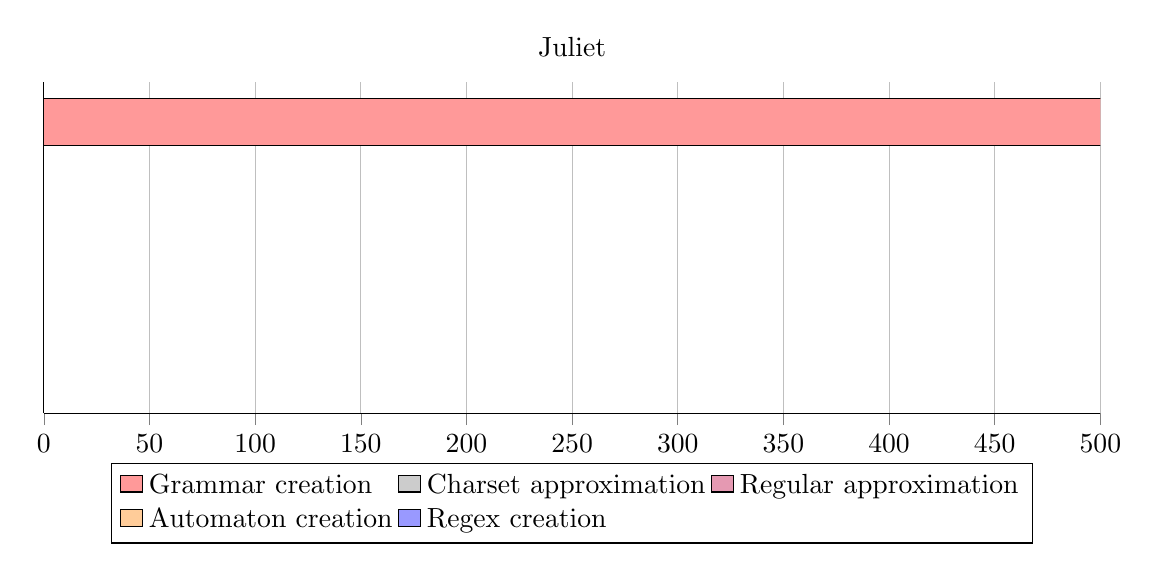
\begin{tikzpicture}
			\begin{axis}[stackedBar,legend style={area legend, at={(0.5,-0.15)}, anchor=north, legend columns=3},legend cell align=left]
				\addplot[fill=red!40] coordinates {(901.1666666666666, 4)};
				\addplot[fill=gray!40] coordinates {(186.56666666666666, 3)};
				\addplot[fill=purple!40] coordinates {(186.83333333333334, 2)};
				\addplot[fill=orange!40] coordinates {(808.6333333333333, 1)};
				\addplot[fill=blue!40] coordinates {(2494.7833333333333, 0)};
				\legend{Grammar creation,Charset approximation,Regular approximation,Automaton creation,Regex creation}
			\end{axis}
		\end{tikzpicture}
	}
	\captionbox{Durations of Tricky example with \ac{dfa} creation in $\mu s$	\label{fig:eval:plot:trickyDFA}}{
		\pgfplotsset{stackedBar/.style={
				title=Tricky with DFA,
				xbar stacked,
				width=15cm,
				axis y line*= none, axis x line*= bottom,
				xmajorgrids = true,
				xmin=0,xmax=5000,
				ytick = \empty,
				yticklabels = {},
				tick align = outside, xtick pos = left,
				bar width=6mm, y=8mm,
				enlarge y limits={abs=0.625},% 0.5 + 0.5*(y - bar width)/y [TeX.sx #47995]
		}}
		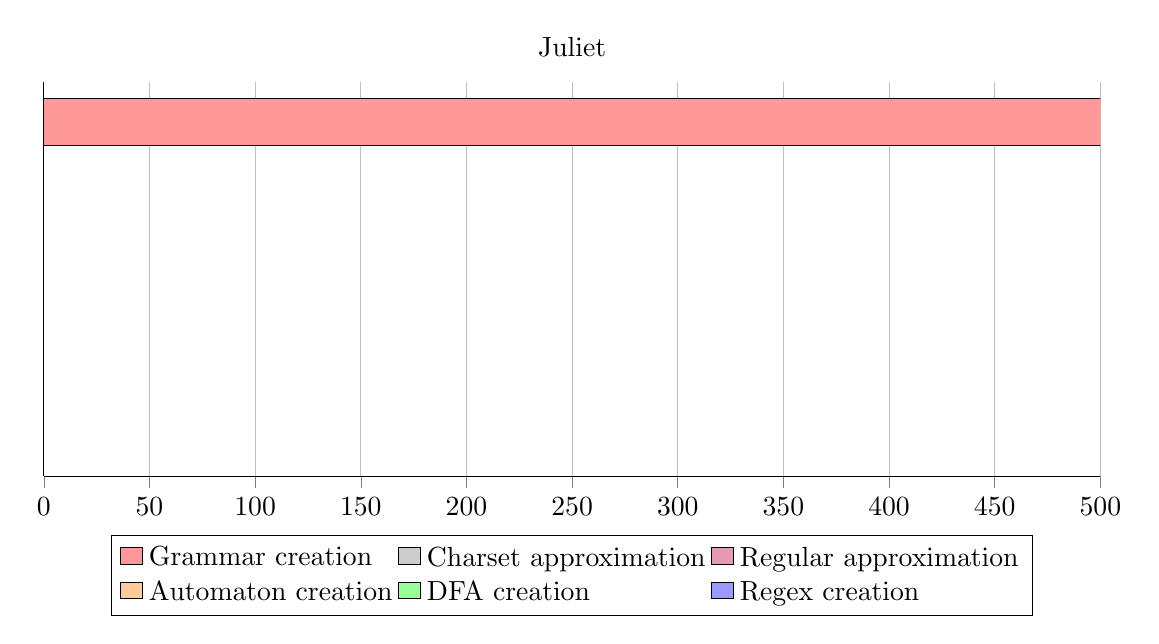
\begin{tikzpicture}
			\begin{axis}[stackedBar,legend style={area legend, at={(0.5,-0.15)}, anchor=north, legend columns=3},legend cell align=left]
				\addplot[fill=red!40] coordinates {(939.9, 5)};
				\addplot[fill=gray!40] coordinates {(197.26666666666668, 4)};
				\addplot[fill=purple!40] coordinates {(192.28333333333333, 3)};
				\addplot[fill=orange!40] coordinates {(910.3666666666667, 2)};
				\addplot[fill=green!40] coordinates {(314.96666666666664, 1)};
				\addplot[fill=blue!40] coordinates {(337.3333333333333, 0)};
				\legend{Grammar creation,Charset approximation,Regular approximation,Automaton creation,DFA creation,Regex creation}
			\end{axis}
		\end{tikzpicture}
	}
\end{figure}

\subsubsection{SQL query sanitization}

Figure \ref{fig:eval:plot:sqlSani} shows the execution time of analyzing the SQL query sanitization example from the previous section. Similar to the Tricky example, the plot shows the average of 100 measurements trimmed by 20\%. 

Note the different scale of the x axis compared to the previous examples. The difference compared to the other plots is explained with the different complexity of the analyzed code. Since the SQL query sanitization example is considerably less complex than the Tricky example, naturally the analysis execution time is lower. 

Figure \ref{fig:eval:plot:sqlSaniDfa} again shows the execution times of the query sanitization example, but with the additional step of creating a \ac{dfa} before performing the state elimination algorithm.

Due to the characteristics of this example, like a simpler data flow, the resulting \ac{nfa} already is a \ac{dfa}. Therefore, the - in this case - unnecessary \ac{dfa} creation just adds additional time, without significantly changing the execution time of the state elimination algorithm. This shows, that whether converting the automaton to a \ac{dfa} improves the execution time is dependent on properties of the input.

\begin{figure}
	\captionbox{Durations of SQL query sanitization test case in $\mu s$\label{fig:eval:plot:sqlSani}}{
		\pgfplotsset{stackedBar/.style={
			title=SQL query sanitization,
			xbar stacked,
			width=15cm,
			axis y line*= none, axis x line*= bottom,
			xmajorgrids = true,
			xmin=0,xmax=2500,
			ytick=\empty,
			yticklabels = {},
			tick align = outside, xtick pos = left,
			bar width=6mm, y=8mm,
			enlarge y limits={abs=0.625},% 0.5 + 0.5*(y - bar width)/y [TeX.sx #47995]
		}}
		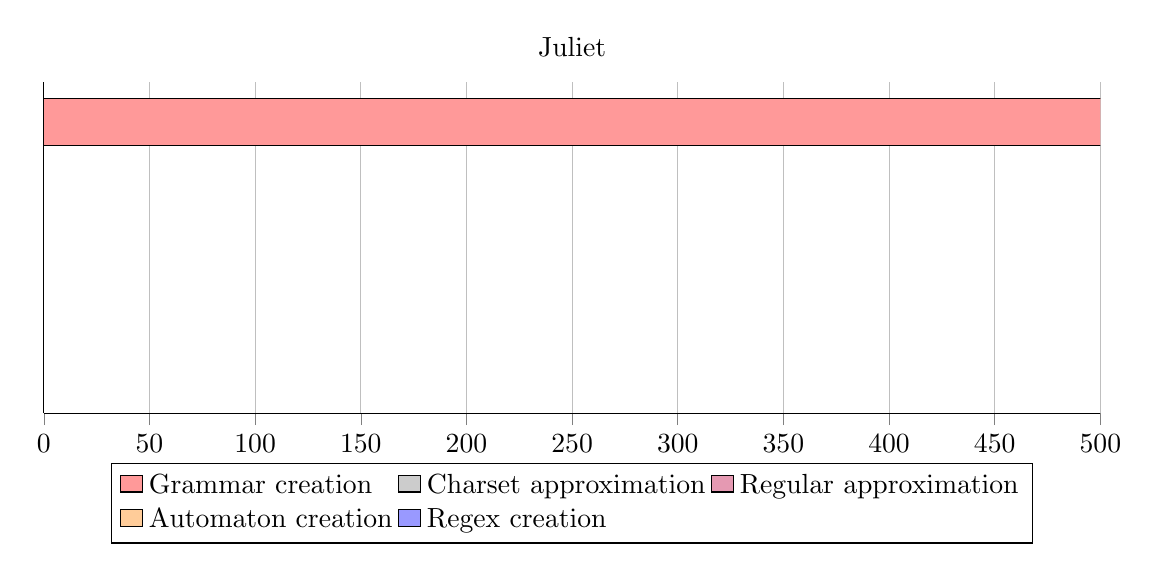
\begin{tikzpicture}
			\begin{axis}[stackedBar,legend style={area legend, at={(0.5,-0.15)}, anchor=north, legend columns=3},legend cell align=left]
				\addplot[fill=red!40] coordinates {(737.6166666666667, 4)};
				\addplot[fill=gray!40] coordinates {(163.65, 3)};
				\addplot[fill=purple!40] coordinates {(72.43333333333334, 2)};
				\addplot[fill=orange!40] coordinates {(480.3, 1)};
				\addplot[fill=blue!40] coordinates {(295.3333333333333, 0)};
				\legend{Grammar creation,Charset approximation,Regular approximation,Automaton creation,Regex creation}
			\end{axis}
		\end{tikzpicture}
	}
		\captionbox{Durations of SQL query sanitization test case with DFA creation in $\mu s$	\label{fig:eval:plot:sqlSaniDfa}}{
		\pgfplotsset{stackedBar/.style={
				title=SQL query sanitization with DFA,
				xbar stacked,
				width=15cm,
				axis y line*= none, axis x line*= bottom,
				xmajorgrids = true,
				xmin=0,xmax=2500,
				ytick=\empty,
				yticklabels = {},
				tick align = outside, xtick pos = left,
				bar width=6mm, y=8mm,
				enlarge y limits={abs=0.625},% 0.5 + 0.5*(y - bar width)/y [TeX.sx #47995]
		}}
		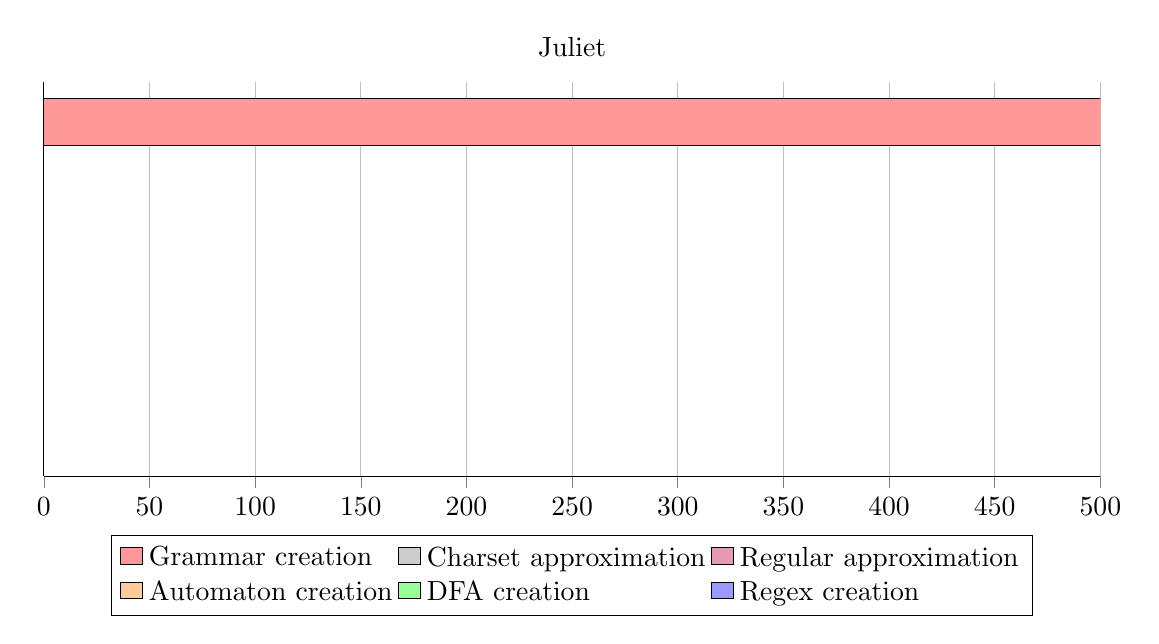
\begin{tikzpicture}
			\begin{axis}[stackedBar,legend style={area legend, at={(0.5,-0.15)}, anchor=north, legend columns=3}, legend cell align=left]
				\addplot[fill=red!40] coordinates {(726.5, 5)};
				\addplot[fill=gray!40] coordinates {(166.48333333333332, 4)};
				\addplot[fill=purple!40] coordinates {(76.36666666666666, 3)};
				\addplot[fill=orange!40] coordinates {(459.1666666666667, 2)};
				\addplot[fill=green!40] coordinates {(117.43333333333334, 1)};
				\addplot[fill=blue!40] coordinates {(288.3333333333333, 0)};
				\legend{Grammar creation,Charset approximation,Regular approximation,Automaton creation,DFA creation,Regex creation}
			\end{axis}
		\end{tikzpicture}
	}
\end{figure}

\subsubsection{Juliet}

We analyzed the execution time of each database related hotspot of all 2224 test cases in the Juliet test suite targeting SQL Injection vulnerabilities.

Figure \ref{fig:eval:plot:juliet} shows the averaged execution times of each step, again trimmed by 20\%.
We can see, that the percentage of the total time spent on regex creation is lower compared to the plot for the Tricky example in Figure \ref{fig:eval:plot:tricky}, even without the intermediary \ac{dfa} step. This is due to the fact that the resulting automata for the Juliet test cases are very small, ranging from 2 to 4 states, compared to the 28 nodes of the Tricky \ac{nfa}.

Again, note the difference in the scale of the x-axis of factor 10, which shows that the Juliet test cases are analyzed significantly faster due to their lower complexity.

Also note that the relative execution times of the different steps are fairly consistent among all the different examples.


\begin{figure}
	\pgfplotsset{stackedBar/.style={
			title=Juliet,
			xbar stacked,
			width=15cm,
			axis y line*= none, axis x line*= bottom,
			xmajorgrids = true,
			xmin=0,xmax=500,
			ytick=\empty,
			yticklabels = {},
			tick align = outside, xtick pos = left,
			bar width=6mm, y=8mm,
			enlarge y limits={abs=0.625},% 0.5 + 0.5*(y - bar width)/y [TeX.sx #47995]
	}}
	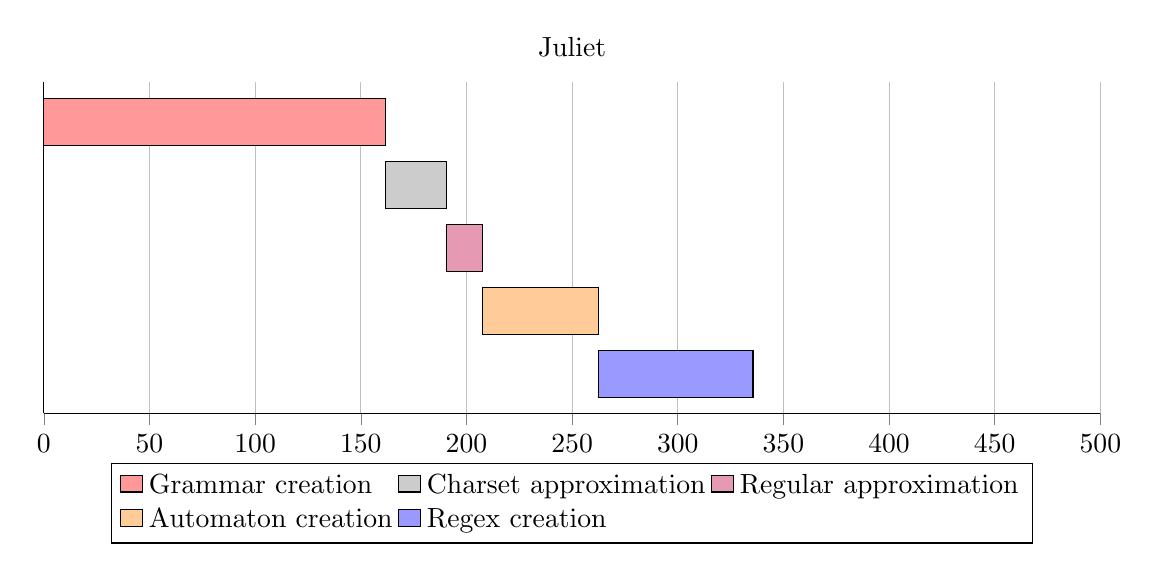
\begin{tikzpicture}
		\begin{axis}[stackedBar,legend style={area legend, at={(0.5,-0.15)}, anchor=north, legend columns=3},legend cell align=left]
			\addplot[fill=red!40] coordinates {(161.81493868450391, 4)};
			\addplot[fill=gray!40] coordinates {(28.68004459308807, 3)};
			\addplot[fill=purple!40] coordinates {(16.914715719063544, 2)};
			\addplot[fill=orange!40] coordinates {(55.07302118171683, 1)};
			\addplot[fill=blue!40] coordinates {(73.1189149015236, 0)};
			\legend{Grammar creation,Charset approximation,Regular approximation,Automaton creation,Regex creation}
		\end{axis}
	\end{tikzpicture}
	\caption{Durations of Juliet test cases in $\mu s$}
	\label{fig:eval:plot:juliet}
\end{figure}

\section{Discussion and Future work}

We discuss several limitations of our implementation and present potential approaches, how future work can mitigate these limitations and extend our implementation.

\subsection{Examples}

We have to note, that all examples we used to test our implementation are synthetic examples. This is due to the fact, that we currently only support a small subset of the Java language, which is not enough to obtain meaningful results from real code. It is unclear how closely the used examples resemble most actual application code and to what extent the observations we made can be transferred to real world use.

\subsection{Assertions}

Our implementation currently does not try to evaluate assertions like \lstinline|s.isEmpty()| due to limitations in the creation of the \ac{cpg} we use.

Consider the example in Listing \ref{lst:assertions} where \lstinline|getSomeKnownValue()| returns some value we can analyze, which is henceforth abbreviated with the generic \lstinline|<val>|.

In our \ac{cpg} the only incoming \ac{dfg} edge of \lstinline|s|$^3$ in line \ref{lst:assertions:ifbody} is an edge from \lstinline|s|$^1$ in line \ref{lst:assertions:def}. However, there is an implicit information flow from \lstinline|s|$^2$ in line \ref{lst:assertions:condition} to \lstinline|s|$^3$, as the result of applying the \lstinline|isEmpty| operation on \lstinline|s|$^2$ influences the information we can get about \lstinline|s|$^3$. If there was a \ac{dfg} edge to the \lstinline|s|$^2$\lstinline|.isEmpty()| call from \lstinline|s|$^3$ instead of the edge from \lstinline|s|$^1$, we could include the operation in our analysis.

For example, for such an edge, we could add a new type of production comparable to the existing operation productions, from the nonterminal representing \lstinline|s|$^3$ to the one representing \lstinline|s|$^2$.

To resolve such an assertion production $A \rightarrow assertion(B)$ we could implement transformations similar to the existing operation productions. For this example, the transformation of the $isEmpty$ assertion would always return just the empty string.
In Listing \ref{lst:assertions}, we could always infer that \lstinline|s|$^3$ is empty, which is clear from the code.

For this example we currently get the regular expression \Verb@(<val>empty)|(<val>)@ as a result. 
Consider \Verb@<val>@ to be \lstinline[mathescape]@abc|$\epsilon$@, which gives us \lstinline[mathescape]@((abc|$\epsilon$)empty)|(abc|$\epsilon$)@.
Here the first part \lstinline[mathescape]@((abc|$\epsilon$)empty)@ corresponds to the value of \lstinline|s|$^4$, which is a possible value of the analyzed \lstinline|s|$^5$ and the second part \lstinline[mathescape]@(abc|$\epsilon$)@ to the value of \lstinline|s|$^1$, which is the result if the condition evaluates to false.

With the mentioned additional \ac{dfg} edges and the described logic, we could sharpen this result.
As mentioned above, the value of \lstinline|s|$^3$ would be $\epsilon$ due to the \lstinline|isEmpty| assertion transformation and therefore \lstinline|s|$^4$ would be a concatenation of $\epsilon$ and the string \lstinline|"empty"|, so just \lstinline|empty|.

This gives us \lstinline[mathescape]@empty|(abc|$\epsilon$)@ as a result, which is more precise, as for example the unobtainable \Verb@abcempty@ is not part of the language of this regular expression.

Similar transformations could also be defined for more complex assertions like \lstinline|s.length() == 1|.

However, as mentioned above, this is currently not possible because the \ac{cpg} is missing the required \ac{dfg} edges representing this implicit information flow from an assertion to subsequent variable usages.

\begin{lstlisting}[caption={Assertion Example}, label=lst:assertions, captionpos=b, float, numbers=right, escapechar=|]
String s|\textcolor{red}{$^1$}| = getSomeKnownValue(); |\label{lst:assertions:def}|
if(s|\textcolor{red}{$^2$}|.isEmpty()){ |\label{lst:assertions:condition}|
	s|\textcolor{red}{$^4$}| = s|\textcolor{red}{$^3$}| + "empty"; |\label{lst:assertions:ifbody}|
}
System.out.println(s|\textcolor{red}{$^5$}|); |\label{lst:assertions:sout}|
\end{lstlisting}

\subsection{Polyvariance}\label{sec:futureWork:polyvariance}

Polyvariance is an analysis strategy, where functions are analyzed more than once, usually once for every call site \cite{polyvariance}. The best result we currently obtain for the Tricky example is the regular expression \Verb@(\()*<int>((\*|\+)<int>\))*@, that does not differentiate between \Verb@*@ and \Verb@+@. Using a polyvariant analysis could improve this, because the two calls to the \lstinline|bar| function would be analyzed separately with respect to their corresponding arguments. Currently, we only follow the \ac{dfg} edges, where the parameter of the function has one to each variable passed as this parameter, here \lstinline|+| and \lstinline|*|. These two edges are not differentiated and the same result is used for both calls to the function.
By differentiating between the corresponding arguments for the analysis of each call, we could sharpen the result to \Verb@\(*<int>(\*<int>\))*(\+<int>\))*@.

\subsection{More extensive implementation}

Currently, the \ac{cpg} does not contain \ac{dfg} edges to differentiate which field of an array is accessed in an array subscription expression like \lstinline|myArray[5]|.

Therefore, we currently do not further analyze values stored in arrays but rather just insert a regular expression generally describing the type stored in the array.

We mostly focused on simple strings, but in general everything we described can be applied to string builders. For example, during grammar creation, a \lstinline|ConcatProduction| could not only be created for \lstinline|s1 + s2| with two strings, but also for \lstinline|sb.append(s)| with a \lstinline|StringBuilder sb| and some other string.

As this is just a proof of concept, we also implemented only a few operations on strings to showcase the approach.

\subsection{State Elimination Heuristics}

Moreira et al. analyzed and evaluated different existing and proposed new heuristics for choosing a good order to eliminate states during the state elimination algorithm \cite{moreira_heuristics}.

While they conclude that the method by Delgado and Morais \cite{delgado} we use is similar to their newly proposed heuristics, they also note that the new strategies outperform Delgado's for small automata. Since the automata we handle are comparatively small, adapting our implementation to use one of the proposed new heuristic could improve the quality of the results.

Moreira et al. also observe that the strategy of taking the best result of using all three heuristics as a final result leads to a gain of 25\%. This approach of trying multiple strategies is also used by the powerful Vcsn platform for computations on finite state machines \cite{vcsn}.

\subsection{Automata Centric Approach}

We chose to provide the information we extracted only as regular expressions due to regular expressions being widely used and supported.
However, representing the information as \acp{dfa} instead of converting the automata to regular expressions has some advantages due to theoretical properties of \acp{dfa}.

Regular expression objects in most programming languages, for example Kotlin's \lstinline|Regex| object, can determine, whether a given string matches the expression. With a sufficiently advanced automaton implementation more advanced checks can be performed.
After analyzing a given hotspot and obtaining an automaton $M$, instead of just matching a given string as a query, the input can be a regular expression. This regular expression can then be turned into another \ac{dfa} $N$.
Since \acp{dfa} are closed under intersection and complement, we can build the \ac{dfa} $R = M \cap \overline{N}$, which accepts words that are in the language of the analysis result, but not in the language of the query expression.
Now we can check, whether $R$'s language is empty to determine, whether all strings of the query are possible values of the analyzed node. Furthermore, if $R$'s language is not empty, we can generate a word from this language as an example for a string that is a possible value of the analyzed node, but not part of the query language.
Additionally, we can check whether $M$ and $N$ are equivalent to determine, whether the query expression matches the computed result.

Since we use \acp{nfa} or optionally already \acp{dfa} as an intermediate representation, future work could increase the capabilities of our automata implementation and implement the mentioned advanced query possibilities.

\begin{comment}
\begin{itemize}
\item How did you test/evaluate your PoC?
    \begin{itemize}
    \item E.g. case studies, large-scale studies, test bench, etc.
    \item What did you do to verify results (if applicable)
    \end{itemize}
\item What did you learn from these tests? Depends on your work. E.g.
    \begin{itemize}
    \item TP/TN/FP/FN rates
    \item Performance
    \item Results of your studies
    \item Interpretation of the results, lessons learned
    \end{itemize}
\item Limitations of the approach and your implementation. Any ideas on how to fix them?
\end{itemize}

Probably 5-15 pages
\end{comment}